\chapter{电力变压器故障诊断方法}

\section{设备结构与诊断信息}
电力变压器由铁芯、绕组、油箱、绝缘套管、冷却装置和保护装置等组成。诊断信息包括设备参数、运行记录、试验结果和检修记录。图\ref{fig:data-management}展示历史示例中的数据管理界面，用于说明信息组织方式。

\begin{figure}[htbp]
  \centering
  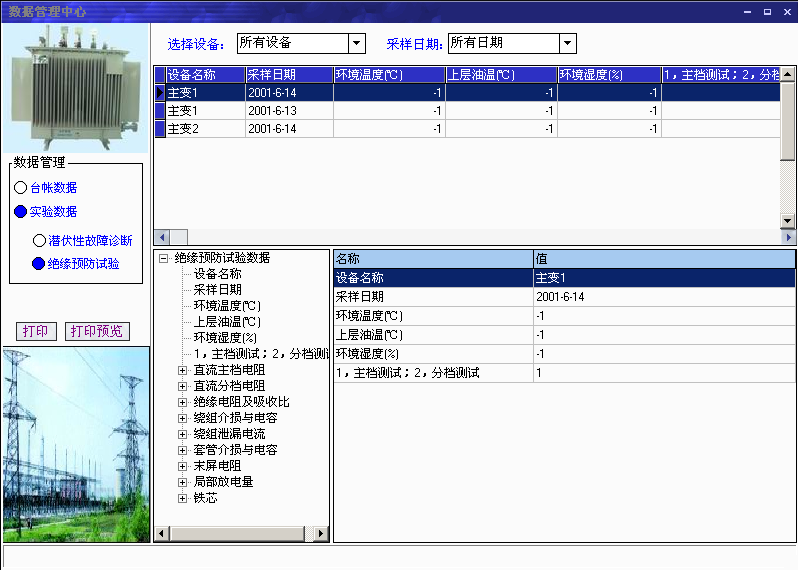
\includegraphics[width=0.85\linewidth]{images/data-management.png}
  \caption{数据管理界面示例}
  \label{fig:data-management}
\end{figure}

\section{故障分类与检测手段}
\subsection{故障分类}
故障可按发生部位划分为内部故障和外部故障。表\ref{tab:faults}列出用于说明分类方式的常见对象。实际分类还应结合具体设备和检测结果。

\begin{table}[htbp]
  \centering
  \caption{按发生部位划分的故障对象}
  \label{tab:faults}
  \begin{tabular}{p{0.42\linewidth}p{0.42\linewidth}}
    \toprule
    内部故障 & 外部故障 \\
    \midrule
    绕组绝缘、导线及连接部位 & 油箱与密封部件 \\
    铁芯及接地部位 & 冷却装置与控制设备 \\
    分接开关及引接线 & 绝缘套管与保护附件 \\
    \bottomrule
  \end{tabular}
\end{table}

\subsection{相对产气速率}
相对产气速率表示一定时间内气体浓度的相对变化，可写为
\begin{equation}
  \gamma_{\mathrm{r}} =
  \frac{C_{i,2}-C_{i,1}}{C_{i,1}}\frac{1}{\Delta t}\times 100\% .
  \label{eq:gas-rate}
\end{equation}

\begin{equationnotes}
  \item[$\gamma_{\mathrm{r}}$] 相对产气速率；
  \item[$C_{i,1}$] 第一次取样测得的第 $i$ 种气体浓度；
  \item[$C_{i,2}$] 第二次取样测得的第 $i$ 种气体浓度；
  \item[$\Delta t$] 两次取样之间的时间间隔。
\end{equationnotes}

式\eqref{eq:gas-rate}要求初始浓度非零，时间单位需保持一致。指标的解释还应考虑设备负荷、取样条件和测量误差。附录给出一组仅用于展示表格排版的数据。
